\chapter{基于属性和并发性的测试}\label{chapt:testing}

本章包括:

\begin{itemize}

\item
  使用QuickCheck进行基于属性的测试
\item
  使用Concuerror检测并发错误
\end{itemize}

在这最后一章(万岁!),我们继续调查一些可用的测试工具。你刚刚看到了ExUnit和Dialyzer。然而,Erlang生态系统还有更多的东西可以提供,正如接下来的部分将展示的那样。

首先,有QuickCheck,这是一个基于属性的测试工具。基于属性的测试将单元测试颠倒过来。与传统的单元测试编写\emph{特定}的测试用例不同,基于属性的测试强迫你以\emph{一般}规范的形式表达你的测试用例。一旦你有了这些规范,这个工具就可以生成你心中期望的尽可能多的测试用例。

接下来,我们将看一下Concuerror。Concuerror是一个系统地检测你的程序中并发错误的工具。Concuerror可以指出难以检测和经常令人惊讶的竞态条件、死锁和潜在的进程崩溃。

本章包含大量的例子供你尝试,提供了充足的机会让你感受这些工具。当你的程序开始变得复杂时,这些工具可以为你的程序提供令人难以置信的洞察力。让我们开始提升我们的测试技能吧!

\section{基于属性的测试和QuickCheck简介}

面对现实 -
单元测试可能是一项艰巨的工作。你经常需要考虑几种情况,并确保覆盖所有的边缘情况。你需要考虑像垃圾数据、极端值和懒惰的程序员只想以最愚蠢的方式通过测试的情况。如果我告诉你,你可以通过编写\emph{规范}来\emph{生成}测试用例,而不是手动编写单个测试用例,你会怎么想?这就是基于属性的测试的全部内容。

下面是一个快速的例子:假设我们正在测试一个排序函数。在单元测试领域,我们会想出不同的列表示例,如:

\begin{enumerate}
  \item \texttt{[3, 2, 1, 5, 4]}
  \item \texttt{[3, 2, 4, 4, 1, 5, 4] \# 有重复的}
  \item \texttt{[1, 2, 3, 4, 5]       \# 已经排序了}
\end{enumerate}


你能想到我们可能遗漏的其他情况吗?在我脑海中,我们遗漏了像空列表和包含负整数的列表这样的情况。说到整数,其他数据类型如原子或元组呢?如你所见,这开始变得繁琐,且遗漏某些边缘情况的概率大大增加。

使用基于属性的测试,我们可以指定排序函数的属性。例如,对列表排序一次与对列表排序两次是一样的。我们可以像这样指定一个属性(暂时不用担心语法):

\begin{code}{代码 11.1 列表排序的一个示例属性}
\begin{minted}[linenos]{elixir}
@tag numtests: 1000
property "sorting twice will yield the same result" do
  forall l <- list(int) do
    ensure(l |> Enum.sort() == l |> Enum.sort() |> Enum.sort())
  end
end
\end{minted}
\label{lst:list_sorting_example_property}
\end{code}

这个属性生成了\emph{一千}种不同的整数列表,并确保这个属性对每个列表都成立。如果属性失败,工具会自动\emph{缩小}测试用例,找到使同一属性失败的最小列表。

我们将要使用的工具是QuickCheck。准确地说,我们将使用Quviq开发的Erlang QuickCheck。虽然Erlang QuickCheck的完整版本需要商业许可,但我们将使用的是一个缩小版的Erlang QuickCheck \emph{Mini}。

\subsubsection{Quviq QuickCheck的付费版和免费版有什么区别?}

两个版本都支持基于属性的测试,这是这个工具的全部要点!付费版本有其他的优点,比如使用状态机进行测试,并行执行测试用例以检测竞态条件(我们将有Conqueror来处理这个问题),当然还有商业支持。

你应该知道,除了Erlang QuickCheck,还有一些类似的基于属性的测试工具可用:

\begin{itemize}

\item  Triform QuickCheck 或 \emph{Triq}\pagenote{http://krestenkrab.github.io/triq}
\item  PropEr\pagenote{https://github.com/manopapad/proper}:  一个受QuickCheck启发的Erlang的基于属性的测试工具
\end{itemize}

Quivq的版本可以说是这三个中最成熟的。虽然免费版本在功能上有些限制,但对我们的目的来说已经足够了。一旦你掌握了基础知识,你可以轻松地转向其他版本的QuickCheck,因为概念是相同的,语法也相似。让我们开始在我们的系统上安装QuickCheck。

\subsection{安装 QuickCheck}

安装 QuickCheck 比通常的 Elixir 依赖稍微复杂一些,但并不困难。首先,前往
Quviq\pagenote{http://www.quviq.com/downloads/} 并下载QuickCheck (Mini)的\emph{免费}版本。除非你有有效的许可证,否则你应该下载免费版本,否则你会被提示输入许可证。一旦你下载了文件,就可以按照以下步骤操作:

\begin{itemize}
	\item 解压文件并 \texttt{cd} 进入结果文件夹
	\item 运行 \texttt{iex}
	\item 运行 \texttt{:eqc\_install.install()}
\end{itemize}

如果一切顺利,你会看到:

\begin{code}{}
\begin{minted}[linenos]{elixir}
iex(1)> :eqc\_install.install
Installation program for "Quviq QuickCheck Mini" version 2.01.0.
Installing in directory /usr/local/Cellar/erlang/18.1/lib/erlang/lib.
Installing ["eqc-2.01.0"].
Quviq QuickCheck Mini is installed successfully.
Bookmark the documentation at /usr/local/Cellar/erlang/18.1/lib/erlang/lib/eqc-2.01.0/doc/index.html.``:ok
\end{minted}
% \label{lst:id}
\end{code}

遵循有用的提示将文档添加到书签会是明智的选择。

\subsection{在 Elixir 中使用 QuickCheck}

现在你已经安装了QuickCheck,我们回到了熟悉的领域。让我们创建一个新的项目来玩玩QuickCheck:

\begin{minted}[linenos]{elixir}
mix(new(quickcheck_playground))
\end{minted}

打开\texttt{mix.ex},并添加以下内容:

\begin{code}{设置一个项目以使用 QuickCheck}
\begin{minted}[linenos]{elixir}
defmodule QuickcheckPlayground.Mixfile do
  use Mix.Project

  def project do
    [
      app: :quickcheck_playground,
      version: "0.0.1",
      elixir: "~> 1.2-rc",
      build_embedded: Mix.env() == :prod,
      start_permanent: Mix.env() == :prod,
      # 1
      test_pattern: "*_{test,eqc}.exs",
      deps: deps
    ]
  end

  def application do
    [applications: [:logger]]
  end

  defp deps do
    # 2
    [{:eqc_ex, "~> 1.2.4"}]
  end
end

# 1: 为测试指定测试模式。注意 QuickCheck 测试的后缀 ``\_eqc''。
# 2: 添加 Erlang QuickCheck 的 Elixir 包装器。
\end{minted}
\label{lst:set_up_a_project_to_use_quickcheck}
\end{code}


执行 \texttt{mix deps.get}来获取依赖项。接下来让我们试一个例子!

\subsubsection{列表反转 - QuickCheck 的 ``Hello World''}

我们将通过编写一个简单的列表反转属性来确保我们已经正确地设置了一切,即,反转一个列表两次会得到相同的列表。

\begin{code}{}
\begin{minted}[linenos]{elixir}
defmodule ListsEQC do
  use ExUnit.Case
  use EQC.ExUnit

  property "reversing a list twice yields the original list" do
    forall l <- list(int) do
      ensure(l |> Enum.reverse() |> Enum.reverse() == l)
    end
  end
end
\end{minted}
% \label{lst:id}
\end{code}

现在不用在意所有这些意味着什么。要运行这个测试,执行
\begin{code}{}
  \begin{minted}[linenos]{elixir}
% mix test test/lists_eqc.exs
    .................................................................................................... 
    OK, passed 100 tests .   
    Finished in 0.06 seconds (0.05s on load, 0.01s on tests)
    1 test, 0 failures  
    Randomized with seed 704750
\end{minted}
  % \label{lst:id}
  \end{code}

太棒了!QuickCheck刚刚运行了\emph{一百}个测试。这是 QuickCheck生成的默认测试数量。
我们可以通过用\texttt{@tag numtests: <N>} 进行注解来修改数量,其中\texttt{<N>}是一个正整数。让我们故意在属性中引入一个错误:


\begin{code}{一个错误的列表反转属性}
\begin{minted}[linenos]{elixir}
defmodule ListsEQC do
  use ExUnit.Case
  use EQC.ExUnit

  property "reversing a list twice yields the original list" do
    forall l <- list(int) do
      # NOTE: THIS IS WRONG!
      ensure(l |> Enum.reverse() == l)
    end
  end
end
\end{minted}
\label{lst:a_wrong_list_reversal_property}
\end{code}

\texttt{ensure/2}检查属性是否满足,并在属性失败时打印出一个错误消息。
让我们再次运行\texttt{mix test test/lists\_eqc.exs} 看看会发生什么:

\begin{code}{QuickCheck 检测到属性中的不一致,并报告一个失败的示例}
  \begin{minted}[linenos]{elixir}
% mix test test/lists_eqc.exs
    ...................Failed! After 20 tests. 
    [0,-2]
    not ensured: [-2, 0] == [0, -2]
    Shrinking xxxx..x(2 times)
    [0,1]
    not ensured: [1, 0] == [0, 1] 
    1) test Property reversing a list twice gives back the original list (ListsEQC) 
    test/lists_eqc.exs:5 
    forall(l <- list(int)) do
    ensure(l |> Enum.reverse() == l)      
    end      
    Failed for [0, 1]        
    stacktrace: 
           test/lists_eqc.exs:5 
      Finished in 0.1 seconds (0.05s on load, 0.06s on tests)
    1 test, 1 failure
\end{minted}
\label{lst:quickcheck_detects_inconsistency_and_reports_a_failing_example}
\end{code}

经过 20 次尝试,QuickCheck报告属性失败,并提供了一个\emph{反例}来支持其声明。
现在我们有信心我们已经正确地设置了QuickCheck,我们可以进入好东西。但首先,你如何设计你自己的属性呢?


\subsection{设计属性的模式}

设计属性是基于属性的测试中最棘手的部分。但不用害怕!这里有一些指针在设计你自己的属性时会很有帮助。当你通过例子学习时,试着找出哪些启发式方法适合。

\subsubsection{反函数}

这是最容易利用的一种。一些函数也有一个反函数。

\begin{figure}[!ht]
    \centering
    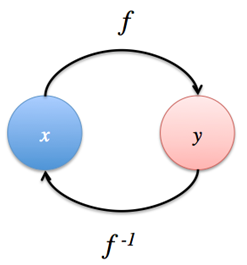
\includegraphics[width=0.8\linewidth]{11_1.png}
    \caption{反函数}
    \label{fig:11_1}
\end{figure}


图\ref{fig:11_1}说明了反函数的含义。主要的思想是反函数撤销了原函数的操作。因此,执行原函数后再执行反函数基本上什么都没做。我们可以利用这个属性来测试二进制的编码和解码,例如使用\texttt{Base.encode64/1} 和\texttt{Base.decode64!} 作为例子:

\begin{code}{编码和解码是彼此的反函数}
\begin{minted}[linenos]{elixir}
property "encoding is the reverse of decoding" do
  forall bin <- binary do
    ensure(bin |> Base.encode64() |> Base.decode64!() == bin)
  end
end
\end{minted}
\label{lst:encoding_is_the_reverse_of_decoding}
\end{code}

你可以尝试执行上述属性,毫无意外,所有的测试都应该通过。这里有一些函数有反函数的更多例子:
\begin{enumerate}
\item  编码和解码
\item  序列化和反序列化
\item  分割和连接
\item  设置和获取
\end{enumerate}

\subsubsection{利用不变性}

另一种技术是利用不变性。不变性是一个在应用特定转换时保持不变的属性。两个不变性的例子:
\begin{enumerate}
\item  排序函数总是按顺序排序元素
\item  单调递增函数总是前一个元素小于或等于下一个元素
\end{enumerate}

假设我们想要测试一个排序函数。首先,我们创建一个辅助函数,检查一个列表是否按递增顺序排序:

\begin{code}{}
\begin{minted}[linenos]{elixir}
def is_sorted([]), do: true

def is_sorted(list) do
  list
  |> Enum.zip(tl(list))
  |> Enum.all?(fn {x, y} -> x <= y end)
end
\end{minted}
% \label{lst:id}
\end{code}

然后我们可以在属性中使用函数来检查排序函数是否正常工作:

\begin{code}{检查排序不变性的属性}
\begin{minted}[linenos]{elixir}
property "sorting works" do
  forall l <- list(int) do
    ensure(l |> Enum.sort() |> is_sorted == true)
  end
end
\end{minted}
\label{lst:checking_the_sorting_invariant}
\end{code}

当你执行上述属性时,一切都应该通过。

\subsubsection{与现有的实现进行比较}

假设你已经开发了一个可以在常数时间内进行排序的排序算法。
测试你的实现的一个简单方法是与一个已知工作良好的\emph{现有}实现进行比较。
例如,我们可以用\emph{Erlang} 的一个来测试我们的自定义实现:

\begin{code}{对现有实现进行测试是保持功能一致性的好方法}
\begin{minted}[linenos]{elixir}
property "List.super_sort/1" do
  forall l <- list(int) do
    ensure(List.super_sort(l) == :lists.sort(l))
  end
end
\end{minted}
\label{lst:testing_against_an_existing_implementation}
\end{code}


\subsubsection{使用更简单的实现}

这是前一种技术的轻微变化。
假设你想要测试一个Map的实现。一种方法是使用一个之前的Map实现。
然而,这可能太麻烦了,而且你的实现的每一个操作可能并不映射到你想要测试的实现。

还有另一种方法!与其使用一个map,为什么不使用像列表这样更简单的东西呢?
是的,它可能不是世界上最高效的数据结构,但它简单,且易于创建map操作的实现。

\begin{figure}[!ht]
    \centering
    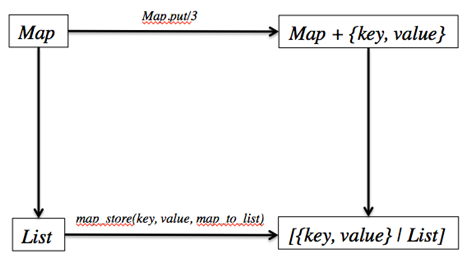
\includegraphics[width=0.8\linewidth]{11_2.png}
    \caption{使用一个更简单的实现来测试一个已经测试过的实现}
    \label{fig:11_2}
\end{figure}


例如,让我们测试一下 \texttt{Map.put/3}操作。
当使用一个已存在的键添加一个值时,旧的值将被替换。
我们如何测试这个呢?让一个例子告诉你:

\begin{code}{使用一个更简单的实现来测试一个更复杂的实现}
\begin{minted}[linenos]{elixir}
property "storing keys and values" do
  forall {k, v, m} <- {key, val, map} do
    map_to_list = m |> Map.put(k, v) |> Map.to_list()
    map_to_list == map_store(k, v, map_to_list)
  end
end

defp map_store(k, v, list) do
  case find_index_with_key(k, list) do
    {:match, index} ->
      List.replace_at(list, index, {k, v})

    _ ->
      [{k, v} | list]
  end
end

defp find_index_with_key(k, list) do
  case Enum.find_index(list, fn {x, _} -> x == k end) do
    nil -> :nomatch
    index -> {:match, index}
  end
end
\end{minted}
\label{lst:using_a_simpler_implementation_to_test_a_more_complex_one}
\end{code}

\texttt{map\_store/3} 辅助函数基本上模拟了\texttt{Map.put/3}会如何添加一个键/值对的行为。
列表包含的元素是两元素元组。元组代表一个键/值对。
当\texttt{map\_store/3}找到匹配键的元组时,它将用相同的键但新的值替换整个元组。
否则,新的键/值被插入到列表中。

在这里,我们正在利用一个事实,即一个map可以被表示为一个列表,而且\texttt{Map.put/3}的行为可以很容易地使用一个列表来实现。
事实上,大多数操作都可以用上面介绍的类似技术来表示(并因此进行测试)。

\subsubsection{执行不同顺序的操作}

对于某些操作,顺序并不重要。这些例子有:
\begin{enumerate}
\item  追加一个列表并反转它,与在列表前面添加一个元素并反转列表是一样的
\item  以不同的顺序向集合中添加元素,不应影响集合中的结果元素
\item 添加一个元素并排序,得到的结果与在元素前面添加一个元素并排序是一样的
\end{enumerate}

\begin{code}{排序的最终结果总是相同的,无论元素在哪里被添加}
\begin{minted}[linenos]{elixir}
property "appending an element and sorting it is the same as prepending an element and sorting it" do
  forall {i, l} <- {int, list} do
    [i | l] |> Enum.sort() == (l ++ [i]) |> Enum.sort()
  end
end
\end{minted}
\label{lst:the_final_result_of_sorting_is_always_the_same_no_matter_where_elements_are_added}
\end{code}

当你执行上述属性时,所有的测试都应该通过。

\subsubsection{幂等操作}

幂等操作是一种花哨的说法,意思是当一个操作执行一次或多次时,它将产生相同的结果。例如:
\begin{enumerate}
\item  使用相同的谓词调用 \texttt{Enum.filter/2}两次,与做一次是一样的
\item  调用 \texttt{Enum.sort/1} 两次,与做一次是一样的
\item  HTTP GET请求
\end{enumerate}

另一个例子是 \texttt{Enum.uniq/2}, 其中调用函数两次不应有任何额外的效果:

\begin{code}{调用一个幂等函数一次或多次总是得到相同的结果}
\begin{minted}[linenos]{elixir}
property "calling Enum.uniq/1 twice has no effect" do
  forall l <- list(int) do
    ensure(l |> Enum.uniq() == l |> Enum.uniq() |> Enum.uniq())
  end
end
\end{minted}
\label{lst:calling_an_idempotent_function_once_or_multiple_times_always_yields_the_same_result}
\end{code}

运行这个属性将通过所有的测试。当然,这六个并不是唯一的,但它们是一个很好的起点。下一个拼图的部分是生成器。让我们直接开始吧。

\subsection{生成器}

生成器用于为我们的QuickCheck属性生成随机测试数据。
这些数据可以是数字(整数,浮点数,实数等),字符串,甚至是不同种类的数据结构,如列表,元组和映射。

在本节中,我们将探索默认情况下可用的生成器。然后,我们将学习如何创建自己的自定义生成器。

\subsubsection{内置生成器}

QuickCheck预装了一堆生成器/生成器组合器。表11.1列出了你可能会遇到的一些更常见的:

\begin{longtable}[]{@{}
  >{\raggedright\arraybackslash}p{(\columnwidth - 2\tabcolsep) * \real{0.5000}}
  >{\raggedright\arraybackslash}p{(\columnwidth - 2\tabcolsep) * \real{0.5000}}@{}}
\toprule()
\begin{minipage}[b]{\linewidth}\raggedright
生成器/组合器
\end{minipage} & \begin{minipage}[b]{\linewidth}\raggedright
描述
\end{minipage} \\
\midrule()
\endhead
\texttt{binary/0} & 生成随机大小的二进制。 \\
\texttt{binary/1} &
生成给定大小(以字节为单位)的二进制。 \\
\texttt{bool/0} & 生成一个随机布尔值。 \\
\texttt{char/0} & 生成一个随机字符。 \\
\texttt{choose/2} & 生成范围在M到N的数字。 \\
\texttt{elements/1} & 生成列表参数的一个元素。 \\
\texttt{frequency/1} &
在其参数中的生成器之间进行加权选择,使得选择每个生成器的概率与其配对的权重成正比。 \\
\texttt{list/1} & 生成由其参数生成的元素的列表。 \\
\texttt{map/2} &
生成一个映射,其中键由K生成,值由V生成。 \\
\texttt{nat/0} &
生成一个小的自然数(受生成大小的限制)。 \\
\texttt{non\_empty/1} & 确保生成的值不为空。 \\
\texttt{oneof/1} &
使用列表生成器的随机选择的元素生成一个值。 \\
\texttt{orderedlist/1} &
生成由G生成的元素的有序列表。 \\
\texttt{real/0} & 生成一个实数。 \\
\texttt{sublist/1} & 生成给定列表的随机子列表。 \\
\texttt{utf8/0} & 生成一个随机utf8二进制。 \\
\texttt{vector/2} &
生成一个给定长度的列表,其中的元素由G生成。 \\
\bottomrule()
\caption{QuickCheck附带的生成器和生成器组合器的列表}
\label{table:11-1}
\end{longtable}


你已经在前面的例子中看到了生成器的应用。以下是使用生成器的一些其他示例。

\begin{example}{指定列表的尾部}

我们如何为获取列表的尾部编写规范呢?作为一个复习,这就是\texttt{tl/1} 的作用:

\begin{code}{tl/1 获取列表的尾部}
\begin{minted}[linenos]{elixir}
iex> h tl          
                           def tl(list) 
    Returns the tail of a list. Raises ArgumentError if the list is empty. 
      Examples 
    ┃ iex> tl([1, 2, 3, :go])
    ┃ [2, 3, :go]”
\end{minted}
\label{lst:tl_1_gets_the_tail_of_a_list}
\end{code}

非空列表的表示形式是 \texttt{[head|tail]},其中\texttt{head}是列表的第一个元素,\texttt{tail}是一个不包含头部的较小列表。
有了这个定义,我们就可以定义属性了:


\begin{code}{获取列表尾部的属性}
\begin{minted}[linenos]{elixir}
property "tail of list" do
  forall l <- list(int) do
    [_head | tail] = l
    ensure(tl(l) == tail)
  end
end
\end{minted}
\label{lst:property_to_get_the_tail_of_a_list}
\end{code}

让我们试试看会发生什么。

\begin{code}{}
\begin{minted}[linenos]{elixir}
1) test Property tail of list (ListsEQC)
test/lists_eqc.exs:11
forall(l <- list(int)) do
[_ | tail] = l
ensure(tl(l) == tail)
end
Failed for []
\end{minted}
% \label{lst:id}
\end{code}

哎呀!原来,QuickCheck找到了一个反例------空列表!
这正好,因为如果你回头看看\texttt{tl/1}的定义,它会在列表为空时引发\texttt{ArgumentError}。
换句话说,我们应该纠正我们的属性。

我们可以尝试使用 \texttt{implies/1}为我们的属性添加一个前提条件。
这里的前提条件将始终确保生成的列表为空。
让我们设置前提条件,我们只想要\emph{非空}的列表:


\begin{code}{使用 implies/2 设置生成列表的前提条件}
\begin{minted}[linenos]{elixir}
property "tail of list" do
  forall l <- list(int) do
    implies l != [] do
      [_head | tail] = l
      ensure(tl(l) == tail)
    end
  end
end
\end{minted}
\label{lst:using_implies_2_to_set_a_precondition_for_the_generated_list}
\end{code}

这次当我们运行测试时,所有的测试都通过了,但我们看到了一些稍微不同的东西:

\begin{code}{}\begin{minted}[linenos]{elixir}
xxxxxxxxxx.xxxxx.xx...x...x...x.(x10)...(x1)xxxxx
OK, passed 100 tests
\end{minted}
\end{code}

交叉符号(\texttt{x})表示一些测试已经被丢弃,因为这些测试没有通过后置条件。
理想情况下,你不希望测试用例被丢弃。
我们可以用不同的方式表达,确保我们生成的列表总是非空的。
在QuickCheck中,我们可以很容易地添加一个生成器组合器,因此摆脱\texttt{implies/1}:

\begin{code}{使用 non\_empty/1 明确生成非空列表}
\begin{minted}[linenos]{elixir}
property "tail of list" do
  forall l <- non_empty(list(int)) do
    [_head | tail] = l
    ensure(tl(l) == tail)
  end
end
\end{minted}
\label{lst:using_non_empty_1_to_explicitly_generate_non_empty_lists}
\end{code}

这次,\emph{没有}测试用例被丢弃:

\begin{minted}[linenos]{elixir}
.................................................................................................... 
OK, passed 100 tests
\end{minted}
\end{example}

\begin{example}{指定列表连接}


到目前为止,我们只使用了一个生成器。有时候,这是不够的。假设我们想要测试\texttt{Enum.concat/2}。
一个直接的方法是测试\texttt{Enum.concat/2} 对比内置的\texttt{++}操作符,它们做的事情是一样的。
这需要两个列表:

\begin{code}{使用多个生成器}
\begin{minted}[linenos]{elixir}
property "list concatenation" do
  forall {l1, l2} <- {list(int), list(int)} do
    ensure(Enum.concat(l1, l2) == l1 ++ l2)
  end
end
\end{minted}
\label{lst:using_multiple_generators}
\end{code}

\end{example}

在下一节中,我们将看到如何定义我们自己的自定义生成器。你会发现QuickCheck的表达能力可以产生我们需要的任何类型的数据。

\subsubsection{创建自定义生成器}

我们一直在使用的所有生成器都是内置的。然而,我们同样可以轻松地创建自己的生成器。
为什么要费这个劲呢?有时候,你希望QuickCheck生成的随机数据具有某些特性。

\begin{example}{指定字符串分割}

假设我们想要测试\texttt{String.split/2}。这个函数接受一个字符串和一个分隔符,并根据分隔符分割字符串。例如:

\begin{code}{}
\begin{minted}[linenos]{elixir}
iex(1) > String.split("everything|is|awesome|!", "|")
["everything", "is", "awesome", "!"]
\end{minted}
% \label{lst:id}
\end{code}

退后一步,思考一下我们可能如何为\texttt{String.split/2}编写一个属性。
一种方法是测试字符串的\emph{逆向}。给定一个函数\texttt{f(x)} 和它的\emph{逆向},
\texttt{f-1(x)},那么我们可以说:

\begin{equation}\label{eq:11_F1}
	f(f^{-1}(x)) = x
\end{equation}

这意味着,当你对一个值应用一个函数,然后对结果值应用逆函数,你会得到原始值。

在这种情况下,使用分隔符分割字符串的逆操作是\emph{连接}分割的结果和相同的分隔符。为此,我们编写了一个快速的辅助函数join,它接受分割操作的标记化结果和分隔符:

\begin{code}{}
\begin{minted}[linenos]{elixir}
def join(parts, delimiter) do
  parts |> Enum.intersperse([delimiter]) |> Enum.join()
end
\end{minted}
% \label{lst:id}
\end{code}

这是一个例子:

\begin{code}{}
\begin{minted}[linenos]{elixir}
iex> join(["everything", "is", "awesome", !], [?|])
"everything|is|awesome|!"
\end{minted}
% \label{lst:id}
\end{code}

有了这个,我们就可以为\texttt{String.split/2}编写一个属性:

\begin{code}{16 使用相同的分隔符分割和连接字符串是逆操作}

\begin{minted}[linenos]{elixir}
defmodule StringEQC do
  use ExUnit.Case
  use EQC.ExUnit

  property "splitting a string with a delimiter and joining it again yields the same string" do
    forall s <- list(char) do
      s = to_string(s)
      ensure(String.split(s, ",") |> join(",") == s)
    end
  end

  defp join(parts, delimiter) do
    parts |> Enum.intersperse([delimiter]) |> Enum.join()
  end
end
\end{minted}
% \label{lst:id}
\end{code}

\texttt{to\\\_string} 在字符列表上

注意使用
\texttt{to\\\_string/1}。这个函数用于将参数转换为字符串,根据
\texttt{String.Chars}
\emph{协议}。本书没有涉及协议,但关键是我们必须将字符列表转换为
\texttt{String.split/2} 可以理解的格式。

然而,有一个小问题。QuickCheck实际上生成包含逗号的字符串的概率是多少呢?让我们用
\texttt{collect/2} 来找出答案:

\begin{code}{17 使用 collect/2,我们可以看到生成数据的分布}

\begin{minted}[linenos]{elixir}
property "splitting a string with a delimiter and joining it again yields the same string" do
forall s <- list(char) do
s = to_string(s)
collect string: s, in:                           #1
ensure String.split(s, ",") |> join(",") == s  #1
end
end

#1: \texttt{collect} 宏报告生成数据的统计信息
\end{minted}
% \label{lst:id}
\end{code}


这是 \texttt{collect/2} 输出的一部分:
\begin{code}{}  \begin{minted}[linenos]{elixir}
1% <<"¡N?½W.E">>
  1% <<121,6,53,194,189,5>>
  1% <<"x2A¤">>
  1% <<"q$">>
  1% <<"g">>
  1% <<102,7,112>>
  1% <<"f">>
  1% <<98,75,6,194,154>>``1% <<"\\¯\e">>
\end{minted}
\end{code}
  

即使你检查整个生成的数据集,你也很难找到包含逗号的东西。
到底有多难呢?QuickCheck有\texttt{classify/3} 可以解决这个问题:

\begin{code}{classify/3 对生成的数据运行一个布尔函数}

\begin{minted}[linenos]{elixir}
property "splitting a string with a delimiter and joining it again yields the same string" do
  forall s <- list(char) do
    s = to_string(s)

    :eqc.classify(
      String.contains?(s, ","),
      :string_with_commas,
      ensure(String.split(s, ",") |> join(",") == s)
    )
  end
end
\end{minted}
% \label{lst:id}
\end{code}

\texttt{classify/3}
对生成的字符串输入和属性运行一个布尔函数,并显示结果。在这种情况下,它报告:

\begin{code}{}\begin{minted}[linenos]{elixir}
....................................................................................................
OK, passed 100 tests
1% string_with_commas
\end{minted}
% \label{lst:id}
\end{code}

虽然所有的测试都通过了,但只有微不足道的\emph{一百分之一}的数据有逗号。由于我们只有一百个测试,所以只有\emph{一个}生成的字符串有一个或多个逗号。

我们真正想要的是生成\emph{更多}包含\emph{更多}逗号的字符串。
幸运的是,QuickCheck给了我们这样做的工具。最终的结果是能够表达这样的属性,其中\texttt{string\_with\_commas}是我们接下来要实现的自定义生成器。

\begin{code}{}
\begin{minted}[linenos]{elixir}
property "splitting a string with a delimiter and joining it again yields the same string" do
  forall s <- string_with_commas do
    s = to_string(s)
    ensure(String.split(s, ",") |> join(",") == s)
  end
end
\end{minted}
% \label{lst:id}
\end{code}

\end{example}


\begin{example}{生成包含逗号的字符串}

让我们为我们的列表提出一些要求。

\begin{enumerate}
	\item 它的长度必须在1到10个字符之间
  \item 字符串应该包含小写字母
  \item 字符串应该包含逗号
  \item 逗号应该比字母出现得少
\end{enumerate}

让我们解决列表中的第一件事。
当使用 \texttt{list/1}生成器时,我们无法控制列表的长度。
为此,我们必须使用\texttt{vector/2} 生成器,它接受一个长度和一个生成器。

在 \texttt{lib}中创建一个新文件\texttt{eqc\_gen.ex}。
让我们从我们的第一个自定义生成器开始:

\begin{code}{vector/2 生成指定长度的列表}
\begin{minted}[linenos]{elixir}
defmodule EQCGen do
  use EQC.ExUnit

  def string_with_fixed_length(len) do
    vector(len, char)
  end
end
\end{minted}
% \label{lst:id}
\end{code}

然后用 \texttt{iex -S mix}打开一个\texttt{iex} 会话。
我们可以用\texttt{:eqc\_gen.sample/1}获取QuickCheck可能生成的样本:

\mintinline{elixir}|iex > :eqc_gen.sample(EQCGen.string\_with\_fixed\_length(5))|

这是一些可能的输出:
\texttt{[170,246,255,153,8]}
\texttt{"ñísJ£"} \texttt{"×¾sûÛ"}
\texttt{"ÈÚwä\\t"}
\texttt{[85,183,155,222,83]}
\texttt{[158,49,169,40,2]}
\texttt{"¥Ùêr¿"}
\texttt{[58,51,129,71,177]}
\texttt{"æ¿q5º"``"C°\{Sð"}

\begin{note}{字符串表示}
请记住,字符串在内部是字符列表,字符可以用整数表示。
\end{note}

生成固定长度的字符串并不好玩。有了\texttt{choose/2},我们可以引入一些变化。


\begin{code}{choose/2 返回一个随机数,我们可以在 vector/2中使用它来生成不同长度的列表}
\begin{minted}[linenos]{elixir}
def string_with_variable_length do
  let len <- choose(1, 10) do
    vector(len, char)
  end
end
\end{minted}
\label{lst:using_choose_2_to_return_a_random_number_we_can_use_in_vector_2_to_generate_lists_of_different_lengths}
\end{code}

这里使用 \texttt{let/2} 很重要。
\texttt{let/2}将生成的值绑定用于另一个生成器。换句话说,这\emph{不会}起作用:


\begin{code}{使用 choose/2 的错误方式。记住 choose/2 也是一个生成器}
\begin{minted}[linenos]{elixir}
# 注意:这不起作用!
def string_with_variable_length do
  vector(choose(1, 10), char)
end
\end{minted}
\label{lst:the_wrong_way_to_use_choose_2_remember_choose_2_is_also_a_generator}
\end{code}

这是因为vector/1的第一个参数应该是一个整数,而不是一个生成器。

\begin{note}{提示:你不必重新启动 iex 会话}
相反,你可以重新编译并重新加载指定模块的源文件。因此,在我们添加了新的生成器后,我们可以直接从会话中重新加载
\begin{code}{}  \begin{minted}[linenos]{elixir}
iex(1)> r(EQCGen)
    lib/eqc_gen.ex:1: warning: redefining module EQCGen
     {:reloaded, EQCGen, [EQCGen]}
\end{minted}
  \end{code}
\end{note}

尝试运行 \texttt{:eqc\_gen.sample/1} 针对\texttt{string\_with\_variable\_length}:

\begin{code}{}\begin{minted}[linenos]{elixir}
iex(1)> :eqc_gen.sample(EQCGen.string_with_variable_length)
  "ß"
  [188,220,86,82,6,14,230,136]
  [150]
  [65,136,250,131,106]
  [4]
  [205,6,254,43,64,115]
  ",ÄØ"
  [184,203,190,93,158,29,250]
  "vp\vwSçú"
  [186,128,49][247,158,120,140,113,186]
\end{minted}
\end{code}

它有效!没有空列表,更长的列表中有十个元素。现在,来解决第二个要求:生成的字符串应该只包含小写字符。关键在于限制字符串中生成的值。目前,我们允许\emph{任何}字符(包括UTF--8)成为字符串的一部分:\texttt{vector(len, char)}

为了达到我们的目标,我们可以使用 \texttt{oneof/1}生成器,它从生成器列表中随机选择一个元素。
在这种情况下,我们只需要提供一个包含小写字母的单一列表。注意我们使用Erlang的\texttt{:lists.seq/2} 函数来生成小写字母的序列:

\mintinline{elixir}|vector(len, oneof(:lists.seq(?a, ?z)))|

重新加载模块并再次运行 \texttt{eqc\_gen.sample/1}:

\mintinline{elixir}|iex > :eqc_gen.sample(EQCGen.string\_with\_variable\_length)|

我们得到了QuickCheck可能生成的一些样本:
\begin{code}{}  \begin{minted}[linenos]{elixir}
"kcra"
"iqtg"
"yqwmqusd"
"hoyacocy"
"jk"
"a"
"iekkoi"
"nugzrdgon"
"tcopskokv"
"wgddqmaq"
"lexsbkosce"
\end{minted}
  \end{code}
  


很好!我们如何在生成的字符串中包含逗号呢?一种方法是简单地将逗号字符作为生成的字符串的一部分:

\mintinline{elixir}|vector(len, oneof(:lists.seq(?a, ?z) ++ [?,]))|

这种方法的问题在于我们无法控制逗号出现的次数。我们可以使用\texttt{frequency/1}来修复这个问题。
在解释之前,先展示一下如何使用\texttt{frequency/1}:

\begin{code}{使用 frequency/1 控制生成值的频率}
  \begin{minted}[linenos]{elixir}
vector(len, frequency([{3, oneof(:lists.seq(?a, ?z))}, {1, ?,}]))
\end{minted}
  \end{code}
  

当我们这样表达时,小写字母将被生成75\%的时间,而逗号将被生成25\%的时间。这是最终的结果:


\begin{code}{使用 frequency/1 增加生成的结果字符串中逗号的概率}
\begin{minted}[linenos]{elixir}
def string_with_commas do
let len <- choose(1, 10) do
vector(len, frequency([{3, oneof(:lists.seq(?a, ?z))},
{1, ?,}]))
end
end
end
\end{minted}
\label{lst:increasing_the_probability_of_commas_in_the_resulting_string_using_frequency_1}
\end{code}

重新加载模块并运行 \texttt{eqc\_gen.sample/1}:

\mintinline{elixir}|iex > :eqc_gen.sample(EQCGen.string\_with\_commas)|
这是生成数据的一个样本:

\begin{code}{}  \begin{minted}[linenos]{elixir}
"acrn" ",,"
  "uandbz,afl" "o,,z"
  ",,wwkr" ",lm"
  ",h,s,aej,"
  ",mpih,vjsq" "swz"
  "n,,yc,""jlvmh,g"
\end{minted}
 \end{code}
  
好多了!现在,让我们使用我们新铸造的生成器:


\begin{code}{使用我们新的生成器,生成包含(更多)逗号的字符串}
\begin{minted}[linenos]{elixir}
property "splitting a string with a delimiter and joining it again yields the same string" do
  # 1
  forall s <- EGCGen.string_with_commas() do
    s = to_string(s)

    :eqc.classify(
      String.contains?(s, ","),
      :string_with_commas,
      ensure(String.split(s, ",") |> join(",") == s)
    )
  end
end

# 1 使用我们新的生成器
\end{minted}
\label{lst:using_our_new_generator_to_generate_strings_with_more_commas}
\end{code}


这次,结果好多了:
\begin{code}{}  \begin{minted}[linenos]{elixir}
....................................................................................................
  OK, passed 100 tests
  65% string_with_commas
\end{minted}
  \end{code}
  

当然,如果你对测试数据的分布仍然不满意,你总是有权力自己调整值。
检查测试数据的分布总是一种好习惯,特别是当你的数据依赖于某些特性,比如至少有一个逗号。
\end{example}

以下是一些你可以尝试实现的生成器示例:
\begin{enumerate}
\item  DNA序列。DNA序列只包含A、T、G和C。例如:\texttt{ACGTGGTCTTAA}。
\item  十六进制序列。十六进制包括0到9,以及字母\texttt{A} 到 \texttt{F}。例如:\texttt{0FF1CE} 和 \texttt{CAFEBEEF}。
\item  排序且唯一的数字序列。例如:\texttt{-4, 10, 12, 35, 100}。
\end{enumerate}

\subsubsection{递归生成器}

让我们尝试一些\emph{稍微}更具挑战性的事情。假设我们需要生成\emph{递归}的测试数据。一个例子是JSON,其中JSON键的值可能是另一个JSON结构。另一个例子是树数据结构(我们将在下一节中看到)。

这就是我们需要\emph{递归}生成器的时候。顾名思义,这些生成器会调用自己。在这个例子中,假设我们要为\texttt{List.flatten/1}编写一个属性,并且我们需要生成嵌套列表。

然而,当使用递归解决问题时,你必须注意不要有无限递归。防止这种情况的方法是让递归调用的输入在每次调用时都变得\emph{更小},并且以某种方式达到一个终止条件。

在QuickCheck中处理递归生成器的标准方法是使用\texttt{sized/2}。\texttt{sized/2}让你可以访问当前正在生成的测试数据的大小参数。我们可以使用这个参数来控制递归调用的输入大小。

\begin{example}{生成任意嵌套的列表(使用List.flatten/2测试)}
\end{example}

举个例子。首先,我们将为我们的测试创建一个入口,以使用嵌套列表生成器:

\begin{code}{sized/2 给我们提供了生成数据的大小参数的访问}
\begin{minted}[linenos]{elixir}
defmodule EQCGen do
  use EQC.ExUnit

  def nested_list(gen) do
    sized size do
      nested_list(size, gen)
    end
  end

  # nested_list/2 还未实现
end
\end{minted}
\label{lst:sized_2_gives_us_access_to_the_size_parameter_of_the_generated_data}
\end{code}

\texttt{nested\_list/1}接受一个生成器作为参数,并将其传递给\texttt{sized/2}中的\texttt{nested\_list/2}。\texttt{nested\_list/2}接受两个参数。\texttt{size}是由\texttt{gen}生成的当前测试数据的大小,而第二个参数是生成器。

我们现在需要实现\texttt{nested\_list/2}。对于列表,有两种情况。列表要么是空的,要么不是。如果传入的大小为零,则应返回一个空列表:


\begin{code}{实现 nested\_list/2 的空列表情况}
\begin{minted}[linenos]{elixir}
defmodule EQCGen do
  use EQC.ExUnit

  # nested/1 在这里

  defp nested_list(0, _gen) do
    []
  end
end
\end{minted}
\label{lst:implementing_the_empty_list_case_of_nested_2}
\end{code}

第二种情况是发生动作的地方:


\begin{code}{实现 nested\_list/2 的非空列表情况。这里是递归发生的地方。}
\begin{minted}[linenos]{elixir}
defmodule EQCGen do
  use EQC.ExUnit

  # nested/1 在这里

  # nested/2 空情况在这里

  defp nested_list(n, gen) do
    oneof([[gen | nested_list(n - 1, gen)], [nested_list(n - 1, gen)]])
  end
end
\end{minted}
\label{lst:implementing_the_non_empty_list_case_of_nested_2_here_is_where_the_recursion_happens}
\end{code}

让我们用
\begin{code}{}  \begin{minted}[linenos]{elixir}
iex(1) > :eqc_gen.sample(EQCGen.nested_list(:eqc_gen.int()))
\end{minted}
\end{code}
试试看。这是结果:

\begin{code}{}  \begin{minted}[linenos]{elixir}
[[-10, [-7, [9, [4, [[]]]]]]]
[10, 0, 2, -3, [[-6, [[-2, -1]]]]]
[[8, [[11, [-7, -3, -9, 10, -8, -10]]]]]
[5, 8, [-10, -11, [7, [-4, -10, 0, [5]]]]]
[[-8, -4, 2, 12, -6, 9, 1, [[[12, -4, []]]]]]
[8, [4, 12, [13, -12, [12, 4, [15, 14, [4]]]]]]
[[[[6, [-11, [[-6, [[[[[[-16]]]]]]]]]]]]]
[-7, 13, [15, -13, [-3, [5, 0, [16, -17, [[[[]]]]]]]]]
[18, [[[[[-8, -8, [3, [-12, [18, [13, [[]]]]]]]]]]]]
[[-2, [[[-6, -17, 3, [[-18, [[12, [[[13, 1]]]]]]]]]]]]
[[[[-15, [-17, [[[-16, [[[20, [[[17, 10, []]]]]]]]]]]]]]]
:ok
\end{minted}
  \end{code}
  
万岁!我们成功地生成了一堆嵌套的整数列表。但你有没有注意到生成过程花费了\emph{很长}的时间?问题出在这一行:

\begin{code}{}  \begin{minted}[linenos]{elixir}
oneof([[gen | nested_list(n - 1, gen)], [nested_list(n - 1, gen)]])
\end{minted}
\end{code}
  
发生的事情是,尽管我们说选择\emph{要么}\texttt{[gen|nested\_list(n-1, gen)]},要么\texttt{[nested\_list(n-1, gen)]}。
实际上发生的是,即使我们只需要其中一个,\emph{两个}表达式都被评估了。
我们需要的是使用\emph{惰性求值}。懒惰只评估我们需要的\texttt{oneof/1}的部分。

幸运的是,我们只需要在 \texttt{oneof/1} 周围包裹一个\texttt{lazy/1}:

\begin{code}{}
\begin{minted}[linenos]{elixir}
lazy do
  oneof([[gen | nested_list(n - 1, gen)], [nested_list(n - 1, gen)]])
end
\end{minted}
% \label{lst:id}
\end{code}

这是最终版本:

\begin{code}{}
\begin{minted}[linenos]{elixir}
defmodule EQCGen do
  use EQC.ExUnit

  def nested_list(gen) do
    sized size do
      nested_list(size, gen)
    end
  end

  defp nested_list(0, _gen) do
    []
  end

  defp nested_list(n, gen) do
    lazy do
      oneof([[gen | nested_list(n - 1, gen)], [nested_list(n - 1, gen)]])
    end
  end
end
\end{minted}
% \label{lst:id}
\end{code}

这次,嵌套列表的生成速度飞快。为了让概念深入人心,我们将通过另一个例子。

\begin{example}{生成平衡树}

在这个例子中,我们将学习如何构建一个生成\emph{平衡树}的生成器。作为复习,平衡树的特点是:

\begin{enumerate}
	\item 左右子树的高度相差最多为一
  \item 左右子树都是平衡的
\end{enumerate}

和以前一样,我们首先创建入口点:

\begin{code}{}
\begin{minted}[linenos]{elixir}
defmodule EQCGen do
  use EQC.ExUnit

  def balanced_tree(gen) do
    sized size do
      balanced_tree(size, gen)
    end
  end

  # balanced_tree/2 not implemented yet
end
\end{minted}
% \label{lst:id}
\end{code}

树的终端节点是\emph{叶节点}。这是树构造的基本情况:

\begin{code}{}
\begin{minted}[linenos]{elixir}
defmodule EQCGen do
  use EQC.ExUnit

  # balanced_tree/1 goes here

  def balanced_tree(0, gen) do
    {:leaf, gen}
  end
end
\end{minted}
% \label{lst:id}
\end{code}

注意我们用 \texttt{:leaf}
原子标记叶节点。接下来,我们需要实现节点\emph{不是}叶子的情况:

\begin{code}{}
\begin{minted}[linenos]{elixir}
defmodule EQCGen do
  use EQC.ExUnit

  # balanced_tree/1 goes here

  # balanced_tree/2 leaf node case here

  def balanced_tree(n, gen) do
    lazy do
      {
        :node,
        gen,
        # 1
        balanced_tree(div(n, 2), gen),
        # 1
        balanced_tree(div(n, 2), gen)
      }
    end
  end
end

# 1: 每次递归调用都会将子树的大小减半
\end{minted}
% \label{lst:id}
\end{code}


对于非叶节点,我们用 \texttt{:node}
标记元组,然后是生成器的值。最后,我们递归调用
\texttt{balanced\_tree/2}
两次:一次是左子树,一次是右子树。每次递归调用都会将生成的子树的大小\emph{减半}。这确保我们最终会达到基本情况并终止。

最后,我们用 \texttt{lazy/1}
包裹递归调用,以确保只在需要时调用递归调用。这是最终版本:

\begin{code}{}
\begin{minted}[linenos]{elixir}
defmodule EQCGen do
  use EQC.ExUnit

  def balanced_tree(gen) do
    sized size do
      balanced_tree(size, gen)
    end
  end

  def balanced_tree(0, gen) do
    {:leaf, gen}
  end

  def balanced_tree(n, gen) do
    lazy do
      {:node, gen, balanced_tree(div(n, 2), gen), balanced_tree(div(n, 2), gen)}
    end
  end
end
\end{minted}
% \label{lst:id}
\end{code}

我们可以生成一些带有整数生成器的平衡树:

\begin{code}{}
\begin{minted}[linenos]{elixir}
iex > :eqc_gen.sample(EQCGen.balanced_tree(:eqc_gen.int()))
\end{minted}
% \label{lst:id}
\end{code}

这会给我们一个像这样的输出:

\begin{code}{}
\begin{minted}[linenos]{elixir}
{node, 0,
 {node, 8, {node, 8, {node, 8, {leaf, 6}, {leaf, -3}}, {node, 1, {leaf, 5}, {leaf, -7}}},
  {node, 1, {node, -4, {leaf, 8}, {leaf, 3}}, {node, 1, {leaf, -8}, {leaf, 7}}}},
 {node, -4, {node, 6, {node, -1, {leaf, 6}, {leaf, 10}}, {node, 5, {leaf, -6}, {leaf, -3}}},
  {node, -4, {node, 6, {leaf, 3}, {leaf, -1}}, {node, 2, {leaf, 8}, {leaf, 8}}}}}
\end{minted}
% \label{lst:id}
\end{code}

尝试生成这些递归结构:

\begin{itemize}

\item  不平衡的树
\item  JSON
\end{itemize}

\end{example}

\subsection{QuickCheck总结}

QuickCheck的核心思想是编写你的代码的属性,并将测试用例的生成和属性的验证交给工具。
一旦你提出了属性,工具就会处理剩下的部分,并可以轻松地生成数百到数千个测试用例。

另一方面,这并非都是彩虹和独角兽------你需要自己思考属性。
虽然思考属性确实需要你花费大量的思考,但收益是巨大的。
通常,通过属性的思考过程会让你对代码有更深入的理解。

我们已经介绍了足够的基础知识,使你能够编写自己的QuickCheck属性和生成器。
还有其他我们没有探索的(高级)领域,比如测试数据的缩小和状态机的验证。
我会在本章的最后温和地指向一些资源。
现在,我们来看看一个名字颇具野心的工具Concuerror的并发测试。

\section{Concuerror并发测试}

虽然Elixir中的actor并发模型消除了一整类的并发错误,但它绝不是银弹。引入并发错误仍然非常可能(而且非常容易)。
在接下来的例子中,我挑战你只通过肉眼查看代码就找出并发错误。

通过传统的单元测试暴露并发错误也是非常困难的,如果不是完全不足的努力。
Concuerror是一个系统地清除并发错误的工具。
虽然它不能找到每一种并发错误,但它能揭示的错误是非常令人印象深刻的。

我们将学习如何使用Concuerror并利用其能力来揭示难以发现的并发错误。
我保证你会对结果感到惊讶。首先,我们需要安装Concuerror。

\subsection{安装Concuerror}

安装Concuerror很简单。以下是所需的步骤:

\begin{code}{}
\begin{minted}[linenos]{bash}
$ git clone https://github.com/parapluu/Concuerror.git
$ cd Concuerror
$ make
MKDIR ebin
GEN  src/concuerror_version.hrl
DEPS src/concuerror_callback.erl
ERLC src/concuerror_callback.erl
…
GEN  concuerror
\end{minted}
% \label{lst:id}
\end{code}

输出的最后一行是Concuerror程序(一个Erlang脚本),为了方便,你可能希望将其包含到你的\texttt{PATH}中。

将\texttt{concuerror}添加到你的\texttt{PATH}

在Unix系统中,这意味着添加一行像这样的内容:

\begin{code}{}
\begin{minted}[linenos]{bash}
export PATH=$PATH:"/path/to/Concuerror"
\end{minted}
% \label{lst:id}
\end{code}

\subsection{设置项目}

创建一个新项目:

\begin{code}{}
\begin{minted}[linenos]{bash}
mix new concuerror_playground
\end{minted}
% \label{lst:id}
\end{code}

接下来,打开 \texttt{mix.exs} 并确保你添加了粗体的行:

\begin{code}{}
\begin{minted}[linenos]{elixir}
defmodule ConcuerrorPlayground.Mixfile do
  use Mix.Project

  def project do
    [
      app: :concuerror_playground,
      version: "0.0.1",
      elixir: "~> 1.2-rc",
      build_embedded: Mix.env() == :prod,
      start_permanent: Mix.env() == :prod,
      # 1
      elixir_paths: elixirc_paths(Mix.env()),
      # 1
      test_pattern: "*_test.ex*",
      # 1
      warn_test_pattern: nil,
      deps: deps
    ]
  end

  def application do
    [applications: [:logger]]
  end

  defp deps do
    []
  end

  # 1
  defp elixirc_paths(:test), do: ["lib", "test/concurrency"]
  # 1
  defp elixirc_paths(_), do: ["lib"]
end

# 1 这些行是为了让Concuerror测试得以编译。
\end{minted}
% \label{lst:id}
\end{code}



默认情况下,Elixir测试以 \texttt{.exs}结尾。这意味着它们没有被编译。
Concuerror不理解\texttt{.exs} 文件(甚至 \texttt{.ex}文件),因此,我们需要告诉Elixir将这些文件编译成\texttt{.beam}。
为了实现这一点,我们首先修改测试模式以接受\texttt{.ex} 和 \texttt{.exs}文件。
我们还关闭了 \texttt{warn\_test\_pattern}选项,
该选项在 \texttt{test} 目录中有\texttt{.ex} 文件时会发出警告。

最后,我们添加两个 \texttt{elixirc\_path/1} 函数并添加\texttt{elixir\_paths}选项。
这明确地告诉编译器我们希望将 \texttt{lib} 和\texttt{test/concurrency} 中的文件都编译。

在我们继续看示例之前,还有最后一点。Concuerror能够以有用的图表显示其输出。我们稍后会看到几个例子。

输出是一个Graphviz \texttt{.dot}文件。
Graphviz是一个开源的图形可视化软件。它可以通过大多数包管理器或者通过\url{http://www.graphviz.org/}获取。确保Graphviz已经正确安装:

\begin{code}{}
\begin{minted}[linenos]{bash}
% dot -V dot - graphviz version 2.38.0 (20140413.2041)
\end{minted}
% \label{lst:id}
\end{code}

\subsection{Concuerror能检测的错误类型}

Concuerror是如何施展其魔力的呢?该工具对你的代码(通常以测试的形式)进行插桩,并知道哪些点可以进行进程交错。有了这个知识,它就可以系统地搜索并报告它能找到的任何错误。它可以检测到的一些与并发相关的错误包括:

\begin{itemize}

\item  死锁
\item  竞态条件
\item  意外的进程崩溃
\end{itemize}

在接下来的例子中,我们将看到Concuerror能够挑选出的错误类型。

\subsection{死锁}

当两个操作都在等待对方完成,因此都无法进行时,就会发生死锁。当Concuerror发现一个程序状态,其中一个或多个进程被阻塞在
\texttt{receive}
上,并且没有其他进程可用于调度时,它会认为该状态已经死锁。我们将看到两个这样的死锁例子。

\begin{example}{Ping Pong(通信死锁)}

我们从一个简单的例子开始。在 \texttt{lib} 中创建\texttt{ping\_pong.ex}:

\begin{code}{}
\begin{minted}[linenos]{elixir}
defmodule PingPong do
  def ping do
    receive do
      :pong -> :ok
    end
  end

  def pong(ping_pid) do
    send(ping_pid, :pong)

    receive do
      :ping -> :ok
    end
  end
end
\end{minted}
% \label{lst:id}
\end{code}

在 \texttt{test/concurrency}
中创建一个对应的测试文件,命名为
\texttt{ping\_pong\_test.ex}。让我们看看测试:

\begin{code}{}
\begin{minted}[linenos]{elixir}
Code.require_file("../test_helper.exs", __DIR__)

defmodule PingPong.ConcurrencyTest do
  import PingPong

  def test do
    ping_pid = spawn(fn -> ping end)
    spawn(fn -> pong(ping_pid) end)
  end
end
\end{minted}
% \label{lst:id}
\end{code}

测试本身非常简单。我们生成两个进程,一个运行
\texttt{ping/0} 函数,一个运行
\texttt{pong/1} 函数。\texttt{pong}
函数接收 \texttt{ping} 进程的pid。

与ExUnit测试相比,有一些细微的差别。
再次注意,与我们通常的以\texttt{.exs}结尾的测试文件不同,我们通过Concuerror的并发测试需要被编译,因此必须以\texttt{.ex} 结尾。
此外,测试函数本身被命名为\texttt{test/0}。

你稍后会看到,Concuerror期望测试函数\emph{没有元数}(没有参数)。
此外,如果你没有明确提供测试函数名,它会自动寻找\texttt{test/0}。
运行测试稍微复杂一些。首先,我们需要编译测试:

\begin{code}{}
\begin{minted}[linenos]{bash}
% mix test
\end{minted}
% \label{lst:id}
\end{code}

接下来,我们需要运行Concuerror。
我们需要明确告诉Concuerror在哪里找到Elixir、ExUnit以及我们项目的编译后的二进制文件。
我们通过指定路径(\texttt{--pa})并指向相应的\texttt{ebin} 目录来做到这一点:

\begin{code}{}
\begin{minted}[linenos]{bash}
concuerror --pa /usr/local/Cellar/elixir/HEAD/lib/elixir/ebin/ \
--pa /usr/local/Cellar/elixir/HEAD/lib/ex_unit/ebin \
--pa _build/test/lib/concuerror_playground/ebin     \
-m Elixir.PingPong.ConcurrencyTest \
--graph ping_pong.dot \--show_races true
\end{minted}
% \label{lst:id}
\end{code}

然后我们需要告诉Concuerror确切的模块,使用 \texttt{-m}标志。
我们需要说\texttt{Elixir.PingPong.ConcurrencyTest} 而不仅仅是\texttt{PingPong.ConcurrencyTest}。
\texttt{--graph}告诉Concuerror生成Graphviz的输出可视化,\texttt{--show\_races true}告诉Concuerror突出显示竞态条件。

此外,这里还有一个 \texttt{-t} 选项。
这个\texttt{-t}选项和一个值一起告诉Concuerror要执行的测试函数。
如前所述,它默认查找\texttt{test/0}。
如果你想指定自己的测试函数,那么你需要提供\texttt{-t}和相应的测试函数名。
看!Concuerror找到了一个错误:

\begin{code}{}
\begin{minted}[linenos]{bash}
# ... output omitted
Error: Stop testing on first error. (Check '-h keep_going').

Done! (Exit status: warning)Summary: 1 errors, 1/1 interleaving explored
\end{minted}
% \label{lst:id}
\end{code}

这是 \texttt{concuerror\_report.txt} 的输出:

\begin{code}{}
\begin{minted}[linenos]{bash}
Erroneous interleaving 1:
* Blocked at a 'receive' (when all other processes have exited):
P.2 in ping_pong.ex line 11
--------------------------------------------------------------------------------

Interleaving info:
1: P: P.1 = erlang:spawn(erlang, apply, [#Fun<'Elixir.PingPong.ConcurrencyTest'.'-test/0-fun-0-'.0>,[]])
in erlang.erl line 2497
2: P: P.2 = erlang:spawn(erlang, apply, [#Fun<'Elixir.PingPong.ConcurrencyTest'.'-test/0-fun-1-'.0>,[]])
in erlang.erl line 2497
3: P: exits normally
4: P.2: pong = erlang:send(P.1, pong)
in ping_pong.ex line 10
5: Message (pong) from P.2 reaches P.1
6: P.1: receives message (pong)
in ping_pong.ex line 4
7: P.1: exits normally

Done! (Exit status: warning)Summary: 1 errors, 1/1 interleaving explored
\end{minted}
% \label{lst:id}
\end{code}

你可能会想知道
\texttt{P}、\texttt{P.1} 和
\texttt{P.2} 是什么。\texttt{P}
是父进程。\texttt{P.1}
是父进程生成的第一个进程,\texttt{P.2}
是父进程生成的第二个进程。现在,让我们告诉Concuerror生成交错的可视化:

\begin{code}{}\begin{minted}[linenos]{bash}
% dot -Tpng ping_pong.dot > ping_pong.png
\end{minted}
% \label{lst:id}
\end{code}

\texttt{ping\_pong.png} 看起来像这样:

% \begin{figure}[!ht]
    % \centering
    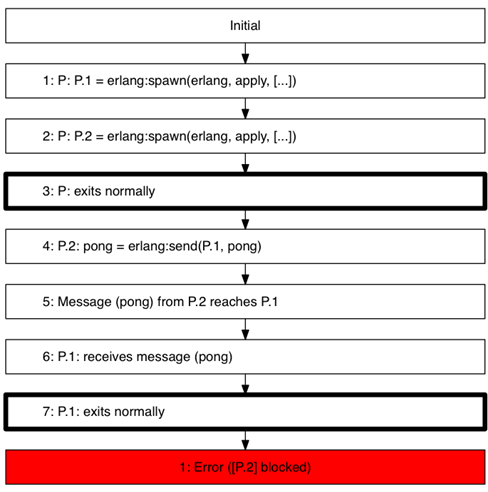
\includegraphics[width=0.8\linewidth]{11_3.png}
    \captionof{figure}{Concuerror显示我们一个被阻塞的进程}
    % \caption{Concuerror显示我们一个被阻塞的进程}
    \label{fig:11_3}
% \end{figure}

\end{example}

报告上的编号行对应图像上的数字。同时查看图像和报告有助于拼凑出导致问题的事件。这就像玩侦探游戏,拼凑犯罪现场的线索!这次,犯罪现场是一个GenServer程序。

\begin{example}{GenServer在另一个同步调用中对自身进行同步调用}

OTP行为可以保护我们免受许多潜在的并发错误,但是很可能会自食其果。下一个例子展示了如何做到这一点。换句话说,不要在家里尝试这个:

\begin{code}{}
\begin{minted}[linenos]{elixir}
defmodule Stacky do
  use GenServer
  require Integer

  @name __MODULE__

  def start_link do
    GenServer.start_link(__MODULE__, :ok, name: @name)
  end

  def add(item) do
    GenServer.call(@name, {:add, item})
  end

  def tag(item) do
    GenServer.call(@name, {:tag, item})
  end

  def stop do
    GenServer.call(@name, :stop)
  end

  def init(:ok) do
    {:ok, []}
  end

  def handle_call({:add, item}, _from, state) do
    new_state = [item | state]
    {:reply, {:ok, new_state}, new_state}
  end

  def handle_call({:tag, item}, _from, state) when Integer.is_even(item) do
    add({:even, item})
  end

  def handle_call({:tag, item}, _from, state) when Integer.is_odd(item) do
    add({:odd, item})
  end

  def handle_call(:stop, _from, state) do
    {:stop, :normal, state}
  end
end
\end{minted}
% \label{lst:id}
\end{code}

数字被添加到Stack GenServer中。如果数字是偶数,那么一个标记的元组
\mintinline{elixir}|{:even, number}|
将被添加到堆栈中。如果是奇数,那么
\mintinline{elixir}|{:odd, number}|
将被推入堆栈。这是\emph{预期的}行为(再次强调,这与当前的实现不符):

\begin{code}{}
\begin{minted}[linenos]{elixir}
iex(1)> Stacky.start_link
{:ok, #PID<0.87.0>}

iex(2)> Stacky.add(1)
{:ok, [1]}

iex(3)> Stacky.add(2)
{:ok, [2, 1]}

iex(4)> Stacky.add(3)
{:ok, [3, 2, 1]}

iex(5)> Stacky.tag(4)
{:ok, [{:even, 4], 3, 2, 1]}

iex(6)> Stacky.tag(5){:ok, [{:odd, 5}, {:even, 4], 3, 2, 1]}
\end{minted}
% \label{lst:id}
\end{code}

不幸的是,当我们尝试 \texttt{Stack.tag/1}
时,我们得到了一个令人讨厌的错误消息:

\begin{code}{}
\begin{minted}[linenos]{bash}
16:44:26.939 [error] GenServer Stacky terminating
** (stop) exited in: GenServer.call(Stacky, {:add, {:even, 4}}, 5000)
** (EXIT) time out
(elixir) lib/gen_server.ex:564: GenServer.call/3
(stdlib) gen_server.erl:629: :gen_server.try_handle_call/4
(stdlib) gen_server.erl:661: :gen_server.handle_msg/5
(stdlib) proc_lib.erl:240: :proc_lib.init_p_do_apply/3
Last message: {:tag, 3}State: [3, 2, 1]
\end{minted}
% \label{lst:id}
\end{code}

花一点时间看看你能否找出问题。在你思考的时候,让Concuerror帮你一点。在
\texttt{test/concurrency} 中创建
\texttt{stacky\_test.ex}。测试很简单:

\begin{code}{}
\begin{minted}[linenos]{elixir}
Code.require_file("../test_helper.exs", __DIR__)

defmodule Stacky.ConcurrencyTest do
  def test do
    {:ok, _pid} = Stacky.start_link()
    Stacky.tag(1)
    Stacky.stop()
  end
end
\end{minted}
% \label{lst:id}
\end{code}

运行\texttt{mix test},然后运行Concuerror看看会发生什么:

\begin{code}{}
\begin{minted}[linenos]{bash}
% concuerror --pa /usr/local/Cellar/elixir/HEAD/lib/elixir/ebin \
--pa /usr/local/Cellar/elixir/HEAD/lib/ex_unit/ebin \
--pa _build/test/lib/concuerror_playground/ebin     \
-m Elixir.Stacky.ConcurrencyTest \--graph stacky.dot
\end{minted}
% \label{lst:id}
\end{code}

这是输出:

\begin{code}{}
\begin{minted}[linenos]{bash}
# output truncated ...
Tip: A process crashed with reason '{timeout, ...}'. This may happen when a call to a gen_server (or similar) does not receive a reply within some standard timeout. Use the '--after_timeout' option to treat after clauses that exceed some threshold as 'impossible'.
Tip: An abnormal exit signal was sent to a process. This is probably the worst thing that can happen race-wise, as any other side-effecting operation races with the arrival of the signal. If the test produces too many interleavings consider refactoring your code.
Info: You can see pairs of racing instructions (in the report and --graph) with '--show_races true'
Error: Stop testing on first error. (Check '-h keep_going').

Done! (Exit status: warning)Summary: 1 errors, 1/2 interleavings explored
\end{minted}
% \label{lst:id}
\end{code}

阅读Concuerror的输出是非常重要的。部分原因是因为Concuerror可能需要你的帮助来进行错误检测。需要注意的是\emph{提示}。让我们从第一个开始:

\begin{code}{}
\begin{minted}[linenos]{bash}
Tip: A process crashed with reason '{timeout, ...}'. This may happen when a call to a gen_server (or similar) does not receive a reply within some standard timeout. Use the '--after_timeout' option to treat after clauses that exceed some threshold as 'impossible'.
\end{minted}
% \label{lst:id}
\end{code}

Concuerror总是假设 \texttt{after}子句是\emph{可能}达到的。
因此,它会搜索那些会触发该子句的交错。然而,由于添加到堆栈是一个相当简单的操作,我们可以明确地告诉Concuerror说
\texttt{after} 子句永远不会被触发,使用
\texttt{--after\_timeout N} 标志,其中任何高于
\texttt{N} 的值都被视为
\texttt{:infinity}。让我们再次运行Concuerror,使用
\texttt{--after\_timeout 1000} 标志:

\begin{code}{}
\begin{minted}[linenos]{bash}
% concuerror --pa /usr/local/Cellar/elixir/HEAD/lib/elixir/ebin \
--pa /usr/local/Cellar/elixir/HEAD/lib/ex_unit/ebin \
--pa _build/test/lib/concuerror_playground/ebin     \
-m Elixir.Stacky.ConcurrencyTest \
--graph stacky.dot \--after_timeout 1000
\end{minted}
% \label{lst:id}
\end{code}

有趣的是,这次没有发出更多的提示。然而,如前所述,Concuerror已经发现了一个错误:

\begin{code}{}
\begin{minted}[linenos]{bash}
% concuerror --pa /usr/local/Cellar/elixir/HEAD/lib/elixir/ebin \
--pa /usr/local/Cellar/elixir/HEAD/lib/ex_unit/ebin \
--pa _build/test/lib/concuerror_playground/ebin     \
-m Elixir.Stacky.ConcurrencyTest \
--graph stacky.dot \--after_timeout 1000

# ... output truncated
Error: Stop testing on first error. (Check '-h keep_going').

Done! (Exit status: warning)
Summary: 1 errors, 1/1 interleavings explored
# ... output truncated
Error: Stop testing on first error. (Check '-h keep_going').

Done! (Exit status: warning)Summary: 1 errors, 1/1 interleavings explored
\end{minted}
% \label{lst:id}
\end{code}

报告揭示了一些关于它找到的错误的细节:

\begin{code}{}
\begin{minted}[linenos]{bash}
Erroneous interleaving 1:
* Blocked at a 'receive' (when all other processes have exited):
P in gen.erl line 168P.1 in gen.erl line 168
\end{minted}
% \label{lst:id}
\end{code}

\texttt{Blocked at a 'receive'}
基本上是Concuerror告诉你发生了死锁。

接下来,它显示了如何发现错误的详细信息:

\begin{code}{}
\begin{minted}[linenos]{bash}
Interleaving info:
1: P: undefined = erlang:whereis('Elixir.Stacky')
in gen.erl line 298
2: P: [] = erlang:process_info(P, registered_name)
in proc_lib.erl line 678
3: P: P.1 = erlang:spawn_opt({proc_lib,init_p,[P,[],gen,init_it,[gen_server,P,P,{local,'Elixir.Stacky'},'Elixir.Stacky',ok,[]]],[link]})
in erlang.erl line 2673
4: P.1: undefined = erlang:put('$ancestors', [P])
in proc_lib.erl line 234
5: P.1: undefined = erlang:put('$initial_call', {'Elixir.Stacky',init,1})
in proc_lib.erl line 235
6: P.1: true = erlang:register('Elixir.Stacky', P.1)
in gen.erl line 301
7: P.1: {ack,P.1,{ok,P.1}} = P ! {ack,P.1,{ok,P.1}}
in proc_lib.erl line 378
8: Message ({ack,P.1,{ok,P.1}}) from P.1 reaches P
9: P: receives message ({ack,P.1,{ok,P.1}})
in proc_lib.erl line 334
10: P: P.1 = erlang:whereis('Elixir.Stacky')
in gen.erl line 256
11: P: #Ref<0.0.1.188> = erlang:monitor(process, P.1)
in gen.erl line 155
12: P: {'$gen_call',{P,#Ref<0.0.1.188>},{tag,1}} = erlang:send(P.1, {'$gen_call',{P,#Ref<0.0.1.188>},{tag,1}}, [noconnect])
in gen.erl line 166
13: Message ({'$gen_call',{P,#Ref<0.0.1.188>},{tag,1}}) from P reaches P.1
14: P.1: receives message ({'$gen_call',{P,#Ref<0.0.1.188>},{tag,1}})
in gen_server.erl line 382
15: P.1: P.1 = erlang:whereis('Elixir.Stacky')
in gen.erl line 256
16: P.1: #Ref<0.0.1.209> = erlang:monitor(process, P.1)
in gen.erl line 155
17: P.1: {'$gen_call',{P.1,#Ref<0.0.1.209>},{add,{odd,1}}} = erlang:send(P.1, {'$gen_call',{P.1,#Ref<0.0.1.209>},{add,{odd,1}}}, [noconnect])in gen.erl line 166
\end{minted}
% \label{lst:id}
\end{code}

最后一行告诉我们导致死锁的行:

\begin{code}{}
\begin{minted}[linenos]{bash}
17: P.1: {'$gen_call',{P.1,#Ref<0.0.1.209>},{add,{odd,1}}} = erlang:send(P.1, {'$gen_call',{P.1,#Ref<0.0.1.209>},{add,{odd,1}}}, [noconnect])
in gen.erl line 166
\end{minted}
% \label{lst:id}
\end{code}

这里的问题是,当两个或更多的同步调用相互等待时,你会得到一个死锁。在这个例子中,同步函数
\texttt{tag/1} 的回调调用了
\texttt{add/1},而 \texttt{add/1}
本身也是同步的。\texttt{tag/1} 会在
\texttt{add/1} 返回时返回,但
\texttt{add/1} 也在等待 \texttt{tag/1}
返回。因此,两个进程都处于死锁状态。

既然我们知道问题出在哪里,那就让我们修复它。需要改变的只是
\texttt{tag/1} 回调函数:

\begin{code}{}
\begin{minted}[linenos]{elixir}
defmodule Stacky do

# ...

def handle_call({:tag, item}, _from, state) when Integer.is_even(item) do
new_state = [{:even, item} |state]
{:reply, {:ok, new_state}, new_state}
end

def handle_call({:tag, item}, _from, state) when Integer.is_odd(item) do
new_state = [{:odd, item} |state]
{:reply, {:ok, new_state}, new_state}
end

# ...end
\end{minted}
% \label{lst:id}
\end{code}

记得编译然后再次运行Concuerror:

\begin{code}{}
\begin{minted}[linenos]{bash}
# ... output omitted
Tip: An abnormal exit signal was sent to a process. This is probably the worst thing that can happen race-wise, as any other side-effecting operation races with the arrival of the signal. If the test produces too many interleavings consider refactoring your code.
Error: Stop testing on first error. (Check '-h keep_going').

Done! (Exit status: warning)Summary: 1 errors, 1/1 interleavings explored
\end{minted}
% \label{lst:id}
\end{code}

哎呀!Concuerror报告了另一个错误。出了什么问题?让我们再次打开报告看看:

\begin{code}{}
\begin{minted}[linenos]{bash}
Erroneous interleaving 1:
* At step 30 process P exited abnormally
Reason:
{normal,{'Elixir.GenServer',call,['Elixir.Stacky',stop,5000]}}
Stacktrace:
[{'Elixir.GenServer',call,3,[{file,"lib/gen_server.ex"},{line,564}]},
{'Elixir.Stacky.ConcurrencyTest',test,0,[{file,"test/concurrency/stacky_test.ex"},{line,8}]}]
\end{minted}
% \label{lst:id}
\end{code}

提示指出了一个异常退出。然而从外表看,我们的GenServer\emph{正常}退出,而
\texttt{Stacky.stop/0}
导致了这个。既然这是Concuerror不应该担心的事情,我们可以安全地告诉它,进程以
\texttt{:normal} 作为原因退出是可以的,使用
\texttt{--treat\_as\_normal normal} 选项:

\begin{code}{}
\begin{minted}[linenos]{bash}
% concuerror --pa /usr/local/Cellar/elixir/HEAD/lib/elixir/ebin \
--pa /usr/local/Cellar/elixir/HEAD/lib/ex_unit/ebin \
--pa _build/test/lib/concuerror_playground/ebin     \
-m Elixir.Stacky.ConcurrencyTest \
--graph stacky.dot \
--show_races true  
--after_timeout 1000 \
--treat_as_normal normal

# ... some output omitted
Warning: Some abnormal exit reasons were treated as normal (--treat_as_normal).
Tip: An abnormal exit signal was sent to a process. This is probably the worst thing that can happen race-wise, as any other side-effecting operation races with the arrival of the signal. If the test produces too many interleavings consider refactoring your code.
Done! (Exit status: completed)Summary: 0 errors, 1/1 interleavings explored
\end{minted}
% \label{lst:id}
\end{code}

万岁!现在一切都好了!
\end{example}


\begin{example}{进程注册的竞态条件}

创建\texttt{lib/spawn\_reg.ex}。
这个例子将演示由进程注册引起的竞态条件。如果你记得,进程注册基本上就是给一个进程分配一个名字。看看下面的实现,看你能否发现竞态条件。

\begin{code}{}
\begin{minted}[linenos]{elixir}
defmodule SpawnReg do
  @name __MODULE__

  def start do
    case Process.whereis(@name) do
      nil ->
        pid = spawn(fn -> loop end)
        Process.register(pid, @name)
        :ok

      _ ->
        :already_started
    end
  end

  def loop do
    receive do
      :stop ->
        :ok

      _ ->
        loop
    end
  end
end
\end{minted}
% \label{lst:id}
\end{code}

这个程序看起来足够无辜。\texttt{start/0}函数创建了一个命名的进程,但在此之前,它会检查是否已经用该名字注册过。
当生成时,进程在接收到\texttt{:stop}消息时终止,并在其他情况下继续愉快地运行。你能找出这个程序的问题吗?

在 \texttt{test/concurrency\_test/spawn\_reg\_test.ex}中创建测试文件。
我们在另一个进程中生成\texttt{SpawnReg} 进程,然后我们告诉\texttt{SpawnReg} 进程停止:

\begin{code}{}
\begin{minted}[linenos]{elixir}
Code.require_file("../test_helper.exs", __DIR__)

defmodule SpawnReg.ConcurrencyTest do
  def test do
    spawn(fn -> SpawnReg.start() end)
    send(SpawnReg, :stop)
  end
end
\end{minted}
% \label{lst:id}
\end{code}

Concuerror发现了一个问题(记得先做一个\texttt{mix test}):

\begin{code}{}
\begin{minted}[linenos]{bash}
% concuerror --pa /usr/local/Cellar/elixir/HEAD/lib/elixir/ebin \
--pa /usr/local/Cellar/elixir/HEAD/lib/ex_unit/ebin \
--pa _build/test/lib/concuerror_playground/ebin     \
-m Elixir.SpawnReg.ConcurrencyTest \
--graph spawn_reg.dot

# ... output omitted
Info: You can see pairs of racing instructions (in the report and --graph) with '--show_races true'
Error: Stop testing on first error. (Check '-h keep_going').

Done! (Exit status: warning)Summary: 1 errors, 1/2 interleavings explored
\end{minted}
% \label{lst:id}
\end{code}

它还告诉我们使用 \texttt{--show\_races true}来揭示竞争指令的对。让我们这样做:

\begin{code}{}
\begin{minted}[linenos]{bash}
% concuerror --pa /usr/local/Cellar/elixir/HEAD/lib/elixir/ebin \
--pa /usr/local/Cellar/elixir/HEAD/lib/ex_unit/ebin \
--pa _build/test/lib/concuerror_playground/ebin     \
-m Elixir.SpawnReg.ConcurrencyTest \
--graph spawn_reg.dot \--show_races true
\end{minted}
% \label{lst:id}
\end{code}

让我们检查一下错误交错的报告:

\begin{code}{}
\begin{minted}[linenos]{bash}
Erroneous interleaving 1:
* At step 3 process P exited abnormally
Reason:
{badarg,[{erlang,send,
['Elixir.SpawnReg',stop],
[9,{file,"test/concurrency/spawn_reg_test.ex"}]}]}
Stacktrace:
[{erlang,send,
['Elixir.SpawnReg',stop],
[9,{file,"test/concurrency/spawn_reg_test.ex"}]}]
* Blocked at a 'receive' (when all other processes have exited):P.1.1 in spawn_reg.ex line 17
\end{minted}
% \label{lst:id}
\end{code}

它告诉我们,在第三步,\texttt{SpawnReg.stop/0}
调用失败,原因是
\texttt{:badarg}。\texttt{P.1.1}
进程也被死锁了。换句话说,它从未收到它正在等待的消息。
\texttt{P.1.1}
是什么进程?这是由父进程生成的第一个进程生成的第一个进程。用更少的话来说:

\begin{code}{}
\begin{minted}[linenos]{elixir}
spawn(fn -> SpawnReg.start() end)
\end{minted}
% \label{lst:id}
\end{code}

Concuerror可能会这样说的另一个原因是我们没有``拆除''我们的进程。一般来说,对于Concuerror测试,一旦我们完成了进程,让它们退出是一种好的做法,比如发送
\texttt{:stop}消息。如果我们检查交错信息,我们可以更好地理解问题:

\begin{code}{}\begin{minted}[linenos]{bash}
Interleaving info:
1: P: P.1 = erlang:spawn(erlang, apply, [#Fun<'Elixir.SpawnReg.ConcurrencyTest'.'-test/0-fun-0-'.0>,[]])
in erlang.erl line 2495
2: P: Exception badarg raised by: erlang:send('Elixir.SpawnReg', stop)
in spawn_reg_test.ex line 9
3: P: exits abnormally ({badarg,[{erlang,send,['Elixir.SpawnReg',stop],[9,{file,[116,101,115,116,47,99,111,110|...]}]}]})
4: P.1: undefined = erlang:whereis('Elixir.SpawnReg')
in process.ex line 359
5: P.1: P.1.1 = erlang:spawn(erlang, apply, [#Fun<'Elixir.SpawnReg'.'-start/0-fun-0-'.0>,[]])
in erlang.erl line 2495
6: P.1: true = erlang:register('Elixir.SpawnReg', P.1.1)
in process.ex line 338
7: P.1: exits normally
--------------------------------------------------------------------------------

Pairs of racing instructions:
*    2: P: Exception badarg raised by: erlang:send('Elixir.SpawnReg', stop)6: P.1: true = erlang:register('Elixir.SpawnReg', P.1.1)
\end{minted}
% \label{lst:id}
\end{code}

Concuerror已经帮助我们发现了一个竞态条件!事实上,它甚至指出了导致这个问题的竞争指令对!你可能会发现图像更有帮助。你还会注意到,图像中包含了一个指向竞争指令对的错误。非常方便!

这是图形版本:

% \begin{figure}[!ht]
%     \centering
%     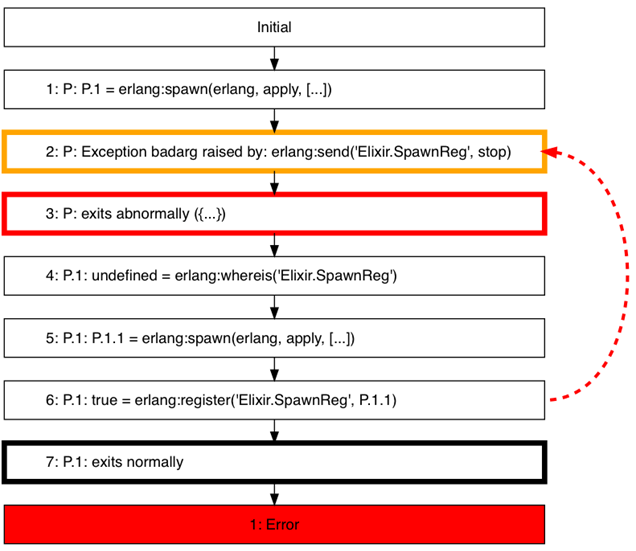
\includegraphics[width=0.8\linewidth]{11_4.png}
%     \caption{Concuerror显示一个竞态条件}
%     \label{fig:11_4}
% \end{figure}


这里的竞态条件发生是因为进程可能还没有完成设置名字。因此,如果\texttt{:name}还没有注册,\texttt{send/2}可能会失败。
Concuerror已经确定这是一个\emph{可能}的交错。如果你在控制台中尝试这个,你很可能甚至没有遇到错误。
\end{example}


\section{Concuerror的总结}

我们刚刚看到了Concuerror可以挑选出的一些并发错误。许多这样的错误并不明显,有时甚至令人惊讶。
使用传统的单元测试技术,几乎不可能暴露出Concuerror相对容易捕获的并发错误。
此外,单元测试工具无法产生导致错误的进程追踪,无论是进程死锁、崩溃还是竞态条件。
Concuerror是我在开发Elixir程序时会密切关注的一个工具。

\section{资源}

这两个工具都是由研究产生的,因此,你最有可能看到的是关于QuickCheck和Concuerror这样的工具的论文,而不是书籍。你正在见证对后者的一次谦逊的尝试。幸运的是,近年来,这两个工具的创建者们已经在会议上进行了演讲和研讨会,这些都可以在网上免费获取。如果你想深入了解QuickCheck和Concuerror,以下是一些你会发现有用的资源:

\begin{itemize}
\item  Software Testing with QuickCheck (John Hughes的论文)
\item  Testing Erlang Data Types with Quviq QuickCheck (Thomas Arts, Laura M.Castro和John Hughes的论文)
\item  Jesper Louis  Anderson有一系列优秀的文章\pagenote{https://medium.com/@jlouis666},他在这些文章中开发了一个QuickCheck模型,用来测试Erlang  18.0中Map的新实现。
\item  使用Concuerror进行并发程序的测试驱动开发 (Alkis Gotovos, Maria Christakis和Konstantinos Sangonas的论文)
\end{itemize}

在本章中,我们看到了两个强大的工具。一个能够生成你想要的尽可能多的测试用例,另一个能够寻找难以发现的并发错误,并可能揭示我们代码中的洞察。总结一下,我们已经学习了:

\begin{itemize}
\item  如何在Elixir中使用QuickCheck和Concuerror(尽管它们最初是为Erlang程序设计的)
\item  如何通过指定比特定单元测试更一般的属性来使用QuickCheck生成测试用例
\item  学习一些指针来提出我们自己的属性
\item  设计自定义生成器来产生我们需要的确切数据
\item  使用Concuerror来检测各种并发错误,如通信死锁、进程死锁和竞态条件
\item  看到了一些并发错误可能发生的例子
\end{itemize}

我们还没有探索所有的特性,一些高级但非常有用的特性被遗漏了。感谢上帝,否则我永远也写不完这本书!然而,本章应该给你提供了进行自己的探索所需要的基础知识和工具。

/printnotes
